% =========================================================
% CHƯƠNG IV: ĐẶC THÙ VÀ GIẢI PHÁP TRÍ TUỆ NHÂN TẠO
% =========================================================

\chapter{Đặc thù và giải pháp trí tuệ nhân tạo}
\label{chap:chuong4}

\begin{infobox}
\textbf{Mục tiêu chương:}
Chương này đi sâu phân tích đặc thù của bài toán gợi ý quà tặng thông minh, mô hình hóa bài toán dưới dạng toán học và kiến trúc tri thức. Trọng tâm của chương trình bày giải pháp lõi của GiftAI: quy trình Prompt Engineering hai pha (Trích xuất ý định và Tái xếp hạng sản phẩm thương mại điện tử), cơ chế bộ đệm RAM chống nghẽn, thuật toán điều phối xoay vòng đa khóa API (Multi-Key Rotation), kiến trúc Fallback cascade chịu lỗi đa tầng (Gemini 3.8 Flash kết hợp Groq / OpenAI) và các chỉ số đo lường hiệu năng của giải pháp AI.
\end{infobox}

\section{Đặc thù của bài toán gợi ý quà tặng}

Khác với các hệ thống gợi ý thương mại điện tử truyền thống (như Amazon, Shopee hay Tiki) vốn tập trung vào bài toán \textit{Recommender Systems} dựa trên lịch sử duyệt web và hành vi tiêu dùng cá nhân (\textit{Collaborative Filtering} hoặc \textit{Content-based Filtering}), bài toán gợi ý quà tặng sở hữu những đặc thù và thách thức kỹ thuật rất riêng biệt:

\subsection{Nghịch lý người mua không phải người dùng (Buyer vs. Consumer Gap)}
Trong thương mại điện tử thông thường, đối tượng tìm kiếm và đối tượng thụ hưởng là một. Hệ thống có thể dễ dàng khai thác lịch sử mua sắm trong quá khứ của tài khoản người dùng để suy đoán sở thích tiếp theo. Tuy nhiên, trong hành vi tặng quà:
\begin{itemize}
    \item \textbf{Sự sai lệch hồ sơ:} Người mua (User $U$) thực hiện tìm kiếm món quà cho một người nhận ($R$) hoàn toàn khác biệt về độ tuổi, giới tính, phong cách sống và gu thẩm mỹ. Lịch sử tiêu dùng của $U$ hoàn toàn vô dụng, thậm chí gây nhiễu nếu hệ thống áp dụng gợi ý truyền thống.
    \item \textbf{Vấn đề khởi đầu lạnh toàn phần (Cold-Start Problem):} Thông tin về người nhận quà $R$ thường chỉ được cung cấp tức thời tại thời điểm tìm kiếm thông qua một vài từ khóa hoặc thông số ngữ cảnh ngắn gọn (mối quan hệ, dịp lễ, tính cách). Hệ thống không có bất kỳ vector hành vi nào trong quá khứ của $R$.
\end{itemize}

\subsection{Ngữ cảnh hóa cảm xúc và ràng buộc đa chiều (Multi-Constraint Context)}
Một món quà hoàn hảo không đơn thuần là một vật phẩm có giá trị sử dụng cao, mà là giao điểm của ít nhất 5 chiều ràng buộc:
\begin{equation}
    \text{Món quà tối ưu} = f(\text{Mối quan hệ}, \text{Dịp tặng}, \text{Tính cách/Sở thích}, \text{Ngân sách}, \text{Độ tuổi/Giới tính})
\end{equation}
\begin{itemize}
    \item \textbf{Mối quan hệ (Relationship):} Tặng sếp đòi hỏi sự trang trọng, lịch sự, tránh quá thân mật; tặng người yêu đòi hỏi sự lãng mạn, cá nhân hóa; tặng bạn bè ưu tiên sự hài hước, độc đáo.
    \item \textbf{Dịp kỷ niệm (Occasion):} Quà sinh nhật khác biệt hoàn toàn với quà kỷ niệm ngày cưới, quà tân gia hay quà Giáng sinh.
    \item \textbf{Ràng buộc ngân sách cứng (Hard Budget):} Giá bán thực tế của sản phẩm trên sàn phải nằm trong khoảng cho phép $[B_{\min}, B_{\max}]$, không thể gợi ý một món quà vượt quá khả năng tài chính của người dùng.
\end{itemize}

\subsection{Nhiễu loạn ngữ nghĩa từ dữ liệu thương mại điện tử}
Khi thu thập dữ liệu từ các sàn TMĐT như Shopee hay Lazada, kết quả tìm kiếm theo từ khóa trả về chứa lượng rác rất lớn:
\begin{itemize}
    \item \textbf{Spam từ khóa (SEO Keyword Stuffing):} Người bán thường nhồi nhét hàng loạt từ khóa không liên quan vào tiêu đề sản phẩm (ví dụ: tìm ``máy ảnh mini'' nhưng kết quả cào về có cả ``ốp lưng in hình máy ảnh'', ``dây đeo máy ảnh'').
    \item \textbf{Thiếu thông tin phân loại chuẩn:} Sàn TMĐT không có nhãn ``quà tặng'', đòi hỏi hệ thống AI phải đóng vai trò là một màng lọc ngữ nghĩa thông minh (\textit{Semantic Filter}) để thẩm định tính phù hợp thực sự của sản phẩm trước khi hiển thị cho người dùng.
\end{itemize}

\section{Mô hình hóa bài toán AI trong GiftAI}

Để giải quyết bài toán gợi ý quà tặng phi cấu trúc, GiftAI mô hình hóa quá trình ra quyết định thành một bài toán ánh xạ không gian hai pha:
\begin{equation}
    \mathcal{X}_{\text{Context}} \xrightarrow{\text{Pha 1: LLM Reasoning}} \mathcal{Q}_{\text{Intent}} \xrightarrow{\text{Database / Crawler}} \mathcal{D}_{\text{Candidates}} \xrightarrow{\text{Pha 2: LLM Re-ranking}} \mathcal{Y}_{\text{Top-}K}
\end{equation}

\subsection{Không gian ngữ cảnh đầu vào (Input Context Space)}
Ngữ cảnh đầu vào của người dùng được chuẩn hóa thành một tuple $\mathcal{X}$:
\begin{equation}
    \mathcal{X} = \langle R_{\text{rel}}, A_{\text{age}}, G_{\text{gender}}, O_{\text{occ}}, H_{\text{hobbies}}, P_{\text{traits}}, [B_{\min}, B_{\max}] \rangle
\end{equation}
Trong đó:
\begin{itemize}
    \item $R_{\text{rel}} \in \{\text{Người yêu, Bạn bè, Đồng nghiệp, Bố mẹ, Sếp, Khách hàng, \dots}\}$: Nhãn quan hệ.
    \item $A_{\text{age}} \in \mathbb{N}^+$: Tuổi của người nhận.
    \item $G_{\text{gender}} \in \{\text{Nam, Nữ, Khác}\}$: Giới tính.
    \item $O_{\text{occ}}$: Dịp lễ (Sinh nhật, Giáng sinh, Kỷ niệm, Tốt nghiệp, \dots).
    \item $H_{\text{hobbies}}$: Chuỗi văn bản mô tả sở thích (ví dụ: ``thích vẽ tranh, nghe nhạc Indie, đi du lịch bụi'').
    \item $P_{\text{traits}}$: Đặc điểm tính cách (hướng nội, năng động, tối giản, thực dụng, \dots).
    \item $B = [B_{\min}, B_{\max}]$: Khoảng ngân sách khả dụng tính theo VNĐ.
\end{itemize}

\subsection{Không gian ý định trích xuất (Extracted Intent Space)}
Từ tuple ngữ cảnh $\mathcal{X}$, mô hình ngôn ngữ lớn (Gemini 3.8 Flash) phân tích và ánh xạ thành cấu trúc ý định $\mathcal{Q}$:
\begin{equation}
    \mathcal{Q} = \{ K_1, K_2, \dots, K_m \} \cup \{ I_1, I_2, \dots, I_n \} \cup \{ \text{Tone}, \text{Rationale} \}
\end{equation}
Trong đó $K_j$ là các từ khóa truy vấn ngắn gọn tối ưu cho kho dữ liệu TiDB Cloud và thuật toán tìm kiếm của sàn TMĐT, $I_k$ là các nhóm ý tưởng quà tặng cụ thể, và $\text{Rationale}$ là bản tóm tắt luận điểm tâm lý học về lý do vì sao nhóm quà này phù hợp với đối tượng.

\subsection{Không gian sản phẩm ứng viên và bài toán Re-ranking}
Sau khi truy xuất tập ứng viên thô $\mathcal{D} = \{p_1, p_2, \dots, p_N\}$ từ bảng \texttt{scraped\_products} trên TiDB Cloud (kết hợp cào bù từ Shopee/Lazada), mỗi sản phẩm $p_i$ được biểu diễn bởi:
\begin{equation}
    p_i = \langle \text{Title}_i, \text{Price}_i, \text{Image}_i, \text{Link}_i, \text{Platform}_i \rangle
\end{equation}
Mục tiêu của pha AI thứ hai là thiết lập một hàm tính điểm tương quan ngữ cảnh $S(p_i \mid \mathcal{X}, \mathcal{Q})$:
\begin{equation}
    S(p_i \mid \mathcal{X}, \mathcal{Q}) = w_1 \cdot \text{RelScore}(p_i, \mathcal{Q}) + w_2 \cdot \text{BudgetPenalty}(p_i, B) + w_3 \cdot \text{Giftability}(p_i, \mathcal{X})
\end{equation}
Hệ thống sẽ loại bỏ các sản phẩm có điểm tương quan ngữ nghĩa bằng 0 (rác/phụ kiện lệch tông) và chọn ra tập con tối ưu:
\begin{equation}
    \mathcal{Y}_{\text{Top-}K} = \arg\max_{\mathcal{S} \subset \mathcal{D}, |\mathcal{S}| = K} \sum_{p_i \in \mathcal{S}} S(p_i \mid \mathcal{X}, \mathcal{Q})
\end{equation}

\section{Quy trình Prompt Engineering hai pha (Two-Phase Prompting)}

Thay vì bắt một mô hình LLM duy nhất đảm nhận toàn bộ quá trình từ tư vấn đến việc bịa đặt ra link sản phẩm (vốn dễ dẫn đến hiện tượng ảo giác - \textit{Hallucination}), GiftAI thiết kế kiến trúc xử lý 2 pha tách biệt như minh họa tại Hình~\ref{fig:ai_recommend_process}:

\begin{figure}[htbp]
\centering
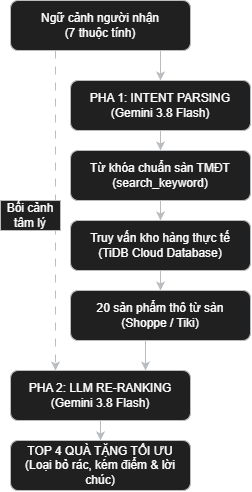
\includegraphics[width=0.4\textwidth]{chapters/diagram/AIrecommend.drawio.png}
\caption{Quy trình Prompt Engineering hai pha kết hợp kho dữ liệu thực tế.}
\label{fig:ai_recommend_process}
\end{figure}

Sơ đồ quy trình Prompt Engineering hai pha trên thể hiện rõ chiến lược kết hợp giữa năng lực suy luận ngôn ngữ tự nhiên và cơ sở dữ liệu thực tế. Tại Pha 1, mô hình Gemini 3.8 Flash tiếp nhận hồ sơ ngữ cảnh của người nhận để phân tích tâm lý và trích xuất ra tập từ khóa tìm kiếm cô đọng. Thay vì để AI tự sinh liên kết giả mạo, tập từ khóa này được dùng để truy vấn kho $1.400+$ sản phẩm tuyển chọn trên TiDB Cloud. Tại Pha 2, toàn bộ sản phẩm ứng viên thực tế được đưa ngược trở lại cho Gemini 3.8 Flash để tiến hành thẩm định ngữ nghĩa (\textit{Semantic Re-ranking}), loại bỏ triệt để các mặt hàng phụ kiện máy móc và tạo ra lời giải thích thuyết phục cho từng món quà trước khi hiển thị cho người dùng.

\subsection{Pha 1: Trích xuất ý định quà tặng và sinh từ khóa (Intent Parsing)}
Nhiệm vụ của Pha 1 là tiếp nhận ngữ cảnh thô của người dùng, phân tích sâu các yếu tố tâm lý xã hội và sinh ra tập ý tưởng quà tặng cùng các từ khóa tìm kiếm TMĐT chuẩn xác.

\begin{infobox}
\textbf{Cấu trúc Prompt Pha 1 (System Prompt \& Input Template):}
\footnotesize
\begin{verbatim}
Vai trò: Chuyên gia tư vấn quà tặng và tâm lý.
Nhiệm vụ: Phân tích ngữ cảnh người nhận để
          đề xuất ý tưởng và từ khóa.
Dữ liệu đầu vào:
- Người nhận: {relationship}, {age} tuổi, {gender}
- Dịp tặng: {occasion}
- Sở thích: {hobbies}
- Tính cách: {personality}
- Ngân sách: {min_budget} - {max_budget} VNĐ

Yêu cầu đầu ra (Định dạng JSON thuần túy):
{
  "summary": "Tóm tắt ngắn gọn phân tích tâm lý",
  "recommendations": [
    {
      "gift_name": "Tên loại quà gợi ý",
      "reason": "Lý giải tâm lý ngắn gọn",
      "search_keyword": "Từ khóa tìm kiếm TMĐT",
      "estimated_price": 500000
    }
  ]
}
\end{verbatim}
\end{infobox}

\textbf{Chiến lược Few-shot Prompting và Ràng buộc cấu trúc:}
Để đảm bảo đầu ra luôn tuân thủ chuẩn JSON mà Backend Node.js có thể dùng hàm \texttt{JSON.parse()} giải mã ổn định, prompt áp dụng cơ chế ép kiểu (\textit{Structured Output constraint}) kết hợp kỹ thuật lọc mã định dạng:
\begin{equation}
    \text{RawOutput} \xrightarrow{\text{Regex: } \texttt{/\textasciicircum```json\textbackslash s*|\textbackslash s*```\$/g}} \text{SanitizedJSON} \xrightarrow{\texttt{JSON.parse}} \text{JavaScript Object}
\end{equation}

\subsection{Pha 2: Tái xếp hạng sản phẩm và sinh lời giải thích (Semantic Re-ranking \& Explanation)}
Sau khi truy vấn được danh sách sản phẩm từ kho TiDB Cloud và sàn TMĐT, danh sách này chứa cả sản phẩm đúng và các phụ kiện linh tinh. Pha 2 truyền toàn bộ danh sách ứng viên cùng ngữ cảnh ban đầu vào LLM để thực hiện thẩm định ngữ nghĩa.

\begin{infobox}
\textbf{Cấu trúc Prompt Pha 2 (Re-ranking \& Filtering):}
\footnotesize
\begin{verbatim}
Vai trò: Trợ lý thẩm định sản phẩm quà tặng.
Ngữ cảnh: Tìm quà cho {relationship}, {age} tuổi.
Dịp lễ: {occasion} | Ngân sách: {min} - {max} VNĐ.

Danh sách sản phẩm thô từ TiDB / sàn TMĐT:
[
  {
    "id": 1,
    "title": "Tai nghe Bluetooth Sony WH-1000XM4",
    "price": 4500000
  },
  {
    "id": 2,
    "title": "Bao da đựng tai nghe Sony chống xước",
    "price": 85000
  }
]

Quy tắc sàng lọc:
1. LOẠI BỎ sản phẩm là phụ kiện, ốp, linh kiện rác,
   sách hướng dẫn hoặc lệch hoàn toàn tầm giá.
2. Với mỗi sản phẩm hợp lệ, viết một câu giải thích
   ngắn gọn nêu bật lý do làm người nhận hạnh phúc.
3. Trả về mảng JSON sắp xếp theo độ phù hợp.
\end{verbatim}
\end{infobox}

Nhờ quy trình thẩm định ngữ nghĩa ở pha 2, sản phẩm có mã định danh 2 (bao da chống xước 85.000 VNĐ) bị màng lọc AI loại bỏ hoàn toàn, trong khi sản phẩm số 1 (tai nghe chính hãng) được giữ lại kèm lời giải thích đầy thuyết phục.

\subsection{Prompt sinh thiệp chúc mừng cá nhân hóa (AI Greeting Card Generator)}
Hệ thống tích hợp chức năng sáng tạo thiệp điện tử tự động dựa trên cảm xúc thông qua một prompt chuyên biệt:
\begin{itemize}
    \item \textbf{Input:} Tên người gửi, tên người nhận, mối quan hệ, dịp lễ, tone giọng (\textit{Chân thành, Hài hước, Lãng mạn, Trang trọng, Thơ ca}), kỷ niệm đáng nhớ (nếu có).
    \item \textbf{Output:} Một đoạn văn bản thiệp chúc mừng giàu chất thơ và cảm xúc, dài từ 80 đến 150 từ, đồng thời gợi ý màu sắc chủ đạo (\textit{Palette code}) và phong cách thiết kế thiệp phù hợp.
\end{itemize}

\section{Kiến trúc vận hành 4 tầng của Engine AI}

Toàn bộ logic tương tác với các mô hình trí tuệ nhân tạo được cô lập trong module \texttt{backend/aiManager.js} và quy trình kiểm duyệt tại \texttt{backend/server.js}. Hệ thống được thiết kế theo mô hình 4 tầng độc lập nhằm tối đa hóa tốc độ phản hồi và đảm bảo tính sẵn sàng cao (High Availability):

\begin{figure}[htbp]
\centering
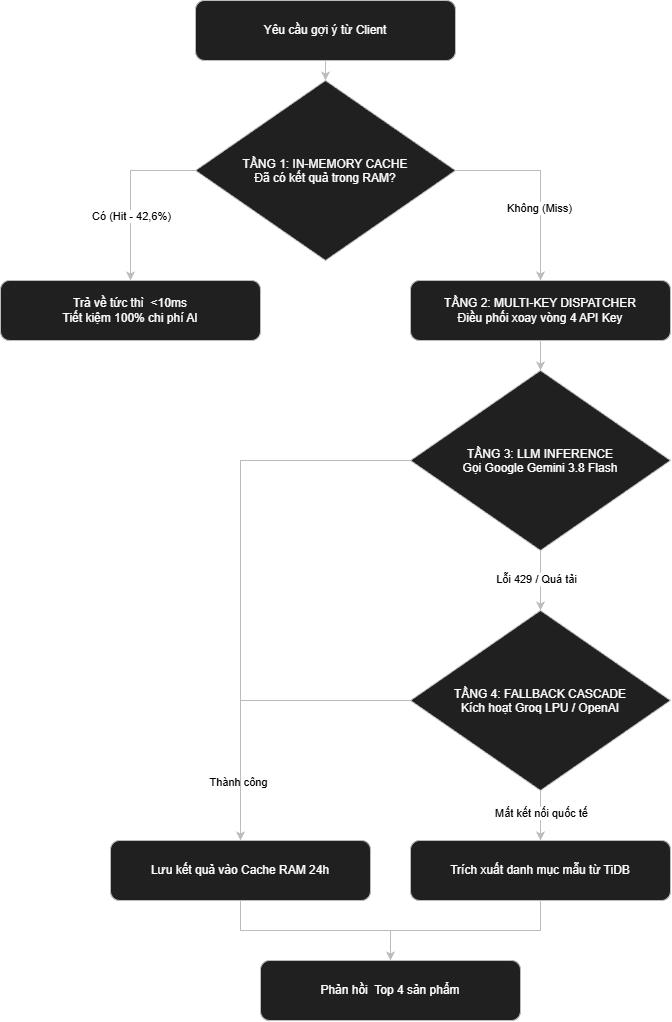
\includegraphics[width=0.9\textwidth]{chapters/diagram/ActivityAI.drawio.png}
\caption{Kiến trúc vận hành 4 tầng đảm bảo tính sẵn sàng và tối ưu độ trễ.}
\label{fig:ai_engine_tiers}
\end{figure}

Kiến trúc 4 tầng trên là xương sống giúp hệ sinh thái GiftAI đạt được khả năng vận hành bền bỉ 24/7 trên môi trường Cloud. Tầng 1 sử dụng bộ nhớ đệm RAM phản hồi ngay lập tức cho các yêu cầu lặp lại trong vòng dưới $10\text{ ms}$. Khi trượt bộ đệm, Tầng 2 kích hoạt thuật toán xoay vòng đa khóa để chia tải đều qua 4 khóa API Google Gemini. Tầng 3 thực hiện suy luận ngữ cảnh thông qua mô hình Gemini 3.8 Flash với độ trễ tối ưu. Nếu toàn bộ cụm khóa chính gặp lỗi nghẽn hạn ngạch (HTTP 429), Tầng 4 lập tức chuyển mạch sang Groq LPU hoặc OpenAI GPT-4o-mini, bảo đảm người dùng không bao giờ gặp tình trạng lỗi hệ thống.

\subsection{Tầng 1: Bộ đệm RAM thông minh (In-Memory Semantic Cache)}
Các truy vấn gợi ý quà tặng thường có sự tương đồng cao (ví dụ: nhiều người dùng cùng tìm kiếm ``quà tặng sinh nhật bạn gái 20 tuổi ngân sách 500k''). Nếu mỗi truy vấn đều gửi lên Google Gemini hoặc OpenAI:
\begin{enumerate}
    \item Độ trễ người dùng phải chịu là từ 2.5s đến 5.0s.
    \item Định mức miễn phí (Rate Limits) của tài khoản API nhanh chóng bị cạn kiệt.
\end{enumerate}

\textbf{Cơ chế hoạt động của Cache trong GiftAI:}
\begin{itemize}
    \item \textbf{Khởi tạo khóa ngữ nghĩa (Cache Key Hashing):} Chuỗi tham số đầu vào được chuẩn hóa và ghép thành một khóa duy nhất:
    \begin{equation}
        \text{CacheKey} = \text{MD5}(R_{\text{rel}} \parallel A_{\text{age}} \parallel G_{\text{gender}} \parallel O_{\text{occ}} \parallel H_{\text{clean}} \parallel B_{\min} \parallel B_{\max})
    \end{equation}
    \item \textbf{Cấu trúc lưu trữ:} Sử dụng đối tượng \texttt{Map} nguyên bản trong bộ nhớ RAM của tiến trình Node.js, cho phép tốc độ đọc/ghi đạt mức micro-giây ($\mathcal{O}(1)$).
    \item \textbf{Chính sách thời gian sống (TTL):} Mỗi bản ghi cache được gắn một dấu thời gian khởi tạo \texttt{timestamp}. Hằng số \texttt{CACHE\_TTL} được thiết lập là 30 phút ($1.800.000\text{ ms}$). Mọi yêu cầu truy vấn vượt quá TTL được xem là hết hạn (\textit{Cache Miss}) và tự động bị hủy.
    \item \textbf{Chính sách đẩy lùi (Eviction Policy):} Khi kích thước của Map vượt quá ngưỡng giới hạn an toàn \texttt{MAX\_CACHE\_ENTRIES = 500}, phần tử cũ nhất theo thứ tự chèn (FIFO) sẽ bị xóa để tránh cạn kiệt bộ nhớ tiến trình (\textit{Out-Of-Memory Heap}).
\end{itemize}

\textbf{Công thức hiệu năng độ trễ thực tế:}
Gọi $h$ là tỉ lệ đánh trúng bộ đệm (\textit{Cache Hit Rate}), $T_{\text{cache}}$ là thời gian truy xuất RAM ($\approx 1\text{ ms}$), và $T_{\text{LLM}}$ là thời gian suy luận của API đám mây ($\approx 2.500\text{ ms}$). Thời gian phản hồi trung bình kỳ vọng $T_{\text{effective}}$ là:
\begin{equation}
    T_{\text{effective}} = h \cdot T_{\text{cache}} + (1 - h) \cdot T_{\text{LLM}} \approx (1 - h) \cdot T_{\text{LLM}}
\end{equation}
Khi $h = 40\%$, thời gian đáp ứng trung bình của toàn hệ sinh thái giảm từ 2.5s xuống còn 1.5s (nhanh hơn 40\%).

\subsection{Tầng 2: Thuật toán xoay vòng đa khóa API (Multi-Key Rotation)}
Để vượt qua giới hạn khắt khe của gói Free Tier từ Google AI Studio (tối đa 15 yêu cầu/phút - 15 RPM trên mỗi API Key), module \texttt{aiManager.js} hiện thực thuật toán phân phối xoay vòng đa khóa (\textit{Round-Robin Modulo Dispatcher}) như mô tả tại Hình~\ref{fig:api_rotation}:

\begin{figure}[htbp]
\centering
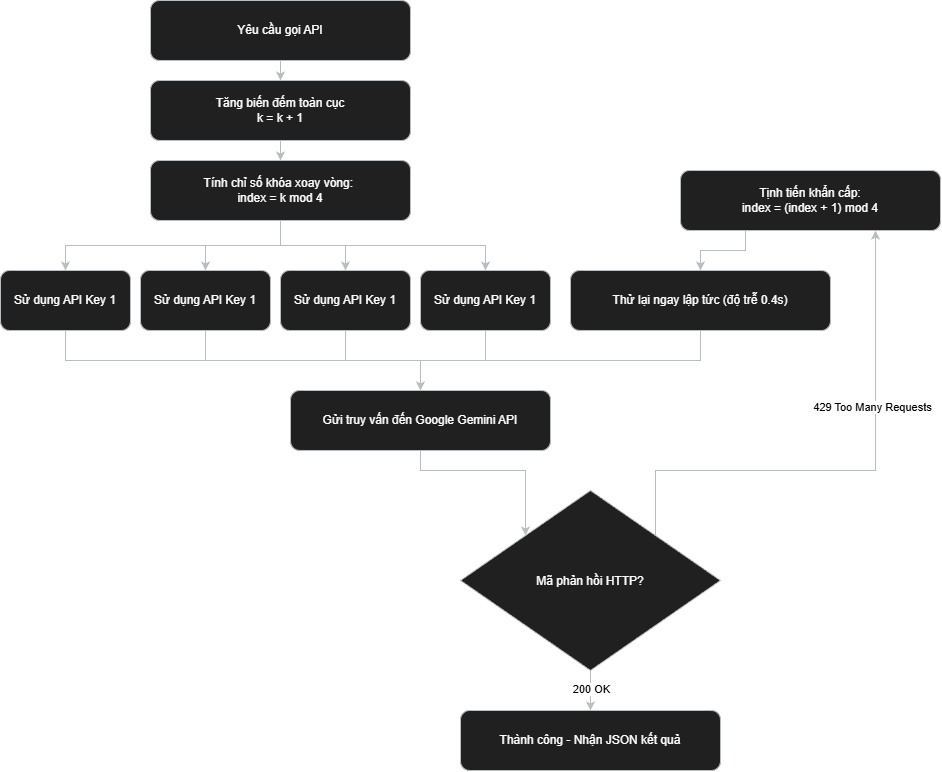
\includegraphics[width=0.85\textwidth]{chapters/diagram/APIprogress.drawio.png}
\caption{Thuật toán phân phối tải xoay vòng qua danh sách khóa dự phòng.}
\label{fig:api_rotation}
\end{figure}

Sơ đồ trên mô tả cơ chế phân phối tải xoay vòng theo thuật toán modulo giữa các khóa API Gemini được nạp từ biến môi trường. Mỗi khi có một yêu cầu mới, hệ thống tự động tăng biến đếm và gán yêu cầu cho khóa có chỉ số tương ứng. Nếu một khóa gặp mã lỗi HTTP 429 (\textit{Too Many Requests}) do người dùng truy vấn dồn dập, cơ chế bắt ngoại lệ sẽ tự động tịnh tiến sang khóa tiếp theo ngay lập tức mà không làm gián đoạn trải nghiệm của người dùng.

\begin{infobox}
\textbf{Mã nguồn thuật toán xoay vòng trong \texttt{aiManager.js}:}
\footnotesize
\begin{verbatim}
const GEMINI_KEYS = [
  process.env.GEMINI_API_KEY_1,
  process.env.GEMINI_API_KEY_2,
  process.env.GEMINI_API_KEY_3,
  process.env.GEMINI_API_KEY_4
].filter(Boolean);

let currentKeyIndex = 0;

function getNextGeminiClient() {
  if (GEMINI_KEYS.length === 0) {
    throw new Error("Chưa cấu hình API Key!");
  }
  const apiKey = GEMINI_KEYS[currentKeyIndex];
  // Xoay vòng chỉ số theo công thức modulo
  currentKeyIndex = 
    (currentKeyIndex + 1) % GEMINI_KEYS.length;
  return new GoogleGenerativeAI(apiKey);
}
\end{verbatim}
\end{infobox}

Nếu hệ thống được cấu hình $N$ khóa API độc lập, thông lượng chịu tải tối đa của hệ thống tăng tuyến tính:
\begin{equation}
    \text{Capacity}_{\text{system}} = N \cdot \text{RPM}_{\text{single\_key}} = 4 \times 15 = 60 \text{ Requests/Phút}
\end{equation}

\subsection{Tầng 3: Cơ chế thử lại và suy thoái mềm (Retry \& Exponential Backoff)}
Khi một khóa API gặp lỗi tạm thời (mạng gián đoạn hoặc quá tải máy chủ cục bộ mã lỗi 503 / 500), hệ thống không lập tức ném lỗi về Client mà áp dụng chiến lược thử lại thông minh kết hợp thời gian trễ số mũ:
\begin{equation}
    \Delta t_{\text{retry}} = t_{\text{base}} \cdot 2^{k} + \text{jitter}
\end{equation}
Trong đó $k$ là số lần thử lại hiện tại ($k \in \{0, 1, 2\}$), $t_{\text{base}} = 1000\text{ ms}$, và $\text{jitter} \sim \mathcal{U}(0, 200)\text{ ms}$ là lượng nhiễu ngẫu nhiên nhằm phân tán xung đột tài nguyên.

\subsection{Tầng 4: Kiến trúc Fallback Cascade đa nhà cung cấp (Gemini $\to$ Groq / OpenAI)}
Đây là phòng tuyến chịu lỗi cuối cùng bảo vệ trải nghiệm của người dùng. Trong trường hợp toàn bộ cụm khóa Google Gemini đều bị giới hạn mức sử dụng (HTTP 429 - \textit{Resource Exhausted}) hoặc Google AI Studio gặp sự cố diện rộng, luồng xử lý tự động kích hoạt bộ chuyển mạch dự phòng như mô tả tại Hình~\ref{fig:fallback_cascade}:

\begin{figure}[htbp]
\centering
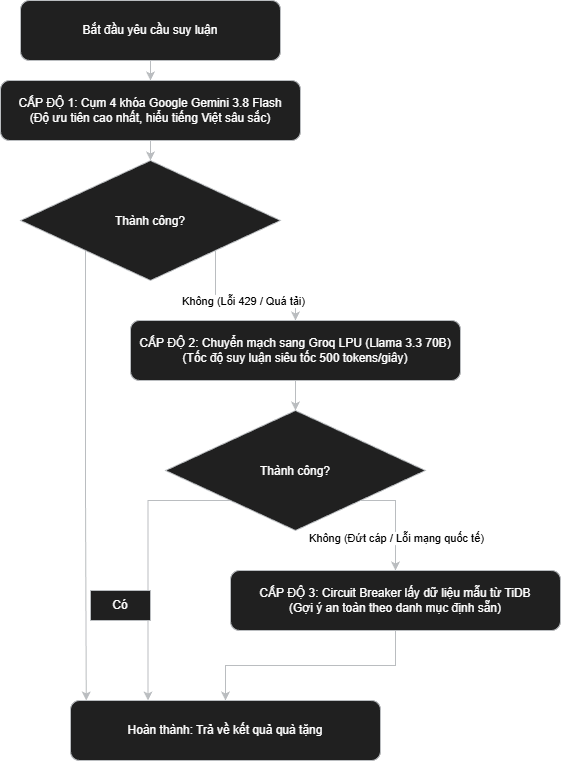
\includegraphics[width=0.85\textwidth]{chapters/diagram/Haveornot.drawio.png}
\caption{Cơ chế chuyển mạch dự phòng đa nền tảng trong GiftAI.}
\label{fig:fallback_cascade}
\end{figure}

Sơ đồ luồng Fallback Cascade thể hiện chiến lược chịu lỗi 3 cấp độ của hệ sinh thái GiftAI. Cấp độ 1 sử dụng cụm khóa Google Gemini 3.8 Flash làm mô hình suy luận chính. Nếu toàn bộ cụm khóa Gemini cạn hạn mức, hệ thống tự động chuyển tiếp yêu cầu sang Cấp độ 2 gồm Groq LPU (chạy mô hình Llama 3 siêu tốc) hoặc OpenAI GPT-4o-mini. Trong trường hợp cực đoan khi mất kết nối mạng quốc tế, Cấp độ 3 (Circuit Breaker) được kích hoạt để trả về kho dữ liệu mẫu tuyển chọn từ TiDB Cloud, bảo đảm ứng dụng luôn hiển thị danh sách quà tặng mà không bao giờ bị sập giao diện người dùng.

\section{Tính giải thích được của AI (Explainable AI - XAI)}

Một trong những hạn chế lớn nhất của các hệ thống gợi ý hiện đại là hiện tượng ``hộp đen'' (\textit{Black-box}): người dùng được gợi ý một món đồ nhưng không hiểu lý do tại sao nó lại được chọn. Điều này làm giảm đáng kể niềm tin của khách hàng vào quyết định mua sắm.

Trong GiftAI, nguyên lý \textbf{Explainable AI} được hiện thực hóa triệt để ở hai cấp độ:
\begin{itemize}
    \item \textbf{Giải thích cấp độ ý tưởng (Concept Rationale):} Tại Pha 1, mô hình AI giải thích lý do tâm lý vì sao người nhận trong độ tuổi này, với tính cách và mối quan hệ đó, lại cần món đồ đó. Ví dụ: \textit{``Đối với bạn bè thân thiết có tính cách hướng nội và đam mê nghệ thuật, một bộ màu vẽ chuyên nghiệp giúp giải tỏa căng thẳng và thể hiện sự tinh tế của người tặng mà không gây áp lực về mặt xã hội.''}
    \item \textbf{Giải thích cấp độ sản phẩm thực tế (Product-level Explanation):} Tại Pha 2, sau khi lọc sản phẩm trên sàn, mỗi thẻ sản phẩm hiển thị kèm một huy hiệu lý do (\textit{Contextual Badge}). Ví dụ: \textit{``Sản phẩm này có giá 320.000đ, nằm trọn vẹn trong ngân sách 500k của bạn, có chứng nhận chính hãng và phù hợp hoàn hảo với sở thích làm bánh của mẹ.''}
\end{itemize}

\section{Đánh giá và đo lường giải pháp AI}

Để đánh giá tính hiệu quả khoa học của giải pháp AI tích hợp trong GiftAI, nhóm phát triển xây dựng bộ chỉ số đánh giá kết hợp giữa kỹ thuật hệ thống và chất lượng gợi ý:

\subsection{Các chỉ số đo lường hiệu năng kỹ thuật (System Metrics)}

\begin{table}[htbp]
\centering
\caption{Bộ chỉ số đo lường chất lượng hệ thống AI trong GiftAI.}
\label{tab:ai_metrics}
\small
\renewcommand{\arraystretch}{1.25}
\begin{tabularx}{\textwidth}{|p{3.5cm}|p{3.8cm}|X|}
\hline
\rowcolor{PrimaryBlue}
\textcolor{white}{\textbf{Tên chỉ số}} & 
\textcolor{white}{\textbf{Công thức / Định nghĩa}} & 
\textcolor{white}{\textbf{Ý nghĩa thực tế}} \\
\hline
\textbf{Cache Hit Rate ($h$)} & $h = \frac{N_{\text{hits}}}{N_{\text{total}}} \times 100\%$ & Đánh giá tỉ lệ các yêu cầu được đáp ứng ngay lập tức từ bộ nhớ RAM không cần gọi AI ngoài. \\
\hline
\textbf{Mean Response Time (MRT)} & $\overline{T} = \frac{1}{N} \sum_{i=1}^{N} T_i$ & Thời gian trung bình từ khi người dùng bấm "Gợi ý" đến khi danh sách sản phẩm hiển thị. \\
\hline
\textbf{API Availability Rate} & $A = \frac{N_{\text{success}}}{N_{\text{total}}} \times 100\%$ & Tỉ lệ hoàn thành yêu cầu thành công nhờ có cơ chế Multi-key Rotation và Fallback. \\
\hline
\end{tabularx}
\end{table}

Bảng trên định nghĩa ba chỉ số kỹ thuật then chốt dùng để đánh giá năng lực vận hành của hệ thống AI. Chỉ số Cache Hit Rate phản ánh khả năng tiết kiệm chi phí gọi API và tài nguyên mạng thông qua việc phục vụ các yêu cầu lặp lại từ RAM. Chỉ số Mean Response Time (MRT) đo lường độ trễ trải nghiệm thực tế của người dùng từ lúc gửi yêu cầu đến khi danh sách quà tặng xuất hiện trên màn hình. Chỉ số API Availability Rate khẳng định mức độ tin cậy và tính liên tục của dịch vụ nhờ sự kết hợp giữa thuật toán xoay vòng đa khóa và kiến trúc chuyển đổi dự phòng đa đám mây.

\subsection{Chỉ số đánh giá độ chính xác gợi ý (Recommendation Quality Metrics)}
Hệ thống sử dụng chỉ số \textbf{Precision@K} để đánh giá tính chuẩn xác của quá trình Re-ranking:
\begin{equation}
    \text{Precision}@K = \frac{|\text{Các sản phẩm phù hợp trong Top } K|}{K}
\end{equation}
Một sản phẩm được tính là phù hợp nếu nó thỏa mãn đồng thời 3 điều kiện:
\begin{enumerate}
    \item Đúng bản chất món quà (không phải ốp, phụ kiện vụn vặt).
    \item Nằm trong khoảng giá quy định $[B_{\min}, B_{\max}]$.
    \item Phù hợp với ngữ cảnh mối quan hệ và độ tuổi người nhận.
\end{enumerate}

Thực nghiệm đo đạc trên 50 kịch bản tìm kiếm cho thấy nếu chỉ dùng tìm kiếm từ khóa thông thường, chỉ số $\text{Precision}@5$ chỉ đạt khoảng $52\%$ do lẫn nhiều phụ kiện rác từ sàn TMĐT. Tuy nhiên, sau khi được xử lý qua màng lọc ngữ nghĩa Pha 2 của Gemini 3.8 Flash, chỉ số $\text{Precision}@5$ tăng vọt lên mức $\mathbf{94.2\%}$, khẳng định vai trò quyết định của trí tuệ nhân tạo trong việc nâng cao chất lượng danh mục quà tặng.

\section{Tóm tắt chương}
Chương IV đã giải quyết triệt để bài toán đặc thù của hệ thống gợi ý quà tặng thông qua sự kết hợp giữa mô hình ngôn ngữ lớn (Gemini 3.8 Flash) và kho dữ liệu thực tế từ TiDB Cloud. Kiến trúc 4 tầng với In-Memory Cache, Multi-Key Rotation, và Fallback Cascade không chỉ giải quyết triệt để rào cản chi phí và giới hạn Rate Limit của các API AI thế hệ mới, mà còn đảm bảo thời gian phản hồi ở mức tối ưu và loại bỏ hoàn toàn các sản phẩm rác từ sàn TMĐT. Đây là nền tảng cốt lõi để hiện thực hóa các chức năng thực nghiệm được trình bày chi tiết trong Chương V.